\subsection{Online Video Games}\label{sec:onlinevideogames}

\emph{League of Legends} (LoL) is a PC game created by \emph{Riot Games} (RG). In the beginning of 2014, LoL had 27 million daily players~\cite{LoL27mill}. One year later, it was the most played multiplayer game~\cite{LoLmostplayed}.

Before a game can start, each player have to create a \emph{summoner}, who has access to \emph{masteries} and \emph{runes} which improves the \emph{champions}. In a classic 5 versus 5 match, 10 players are divided into two competing teams consisting of 5 players each, with the colours blue and purple. Each player will pick a champion to use as their playable character from a pool of 124 different champions. Each champion has 5 unique active abilities of which three are active, one is an ultimate that is extra powerful, and one passive. An \emph{ability} is a magic spell, which does wildly different things, e.g.\ fires a Frost Shot at an opponents champion. 

In \Cref{fig:lolmap}, the map is presented, it consists of three lanes identified as \emph{top}, \emph{middle}, and \emph{bottom} which connects the two bases. The blue and purple colours represent the blue and purple teams' respective structures. Circles are \emph{turrets}, pentagons are \emph{inhibitors} and squares are \emph{nexuses}. The green circle indicates \emph{the dragon} and the pink is \emph{the baron}.

\begin{table}[!h]
  \begin{tabular}{l p{13cm}}
    \textbf{Nexus}: & This building spawn \emph{creeps}, which are small monsters with low damage and health, that walks along each of the lanes toward the opposing teams base. Killing these creeps award \emph{gold} and \emph{experience}. When the nexus is destroyed the game ends, making the destroying team the winners\\
    \textbf{Inhibitor}: & When this is destroyed, the destroying teams' minions become stronger on the lane where the inhibitor was placed\\
    \textbf{Turret}: & This is a defensive structure, which fires at nearby enemies\\
    \textbf{Jungle}: & The area between the lanes which hosts stronger \emph{monsters}\\
  \end{tabular}
\end{table}

\begin{figure}[!htb]
  \centering
    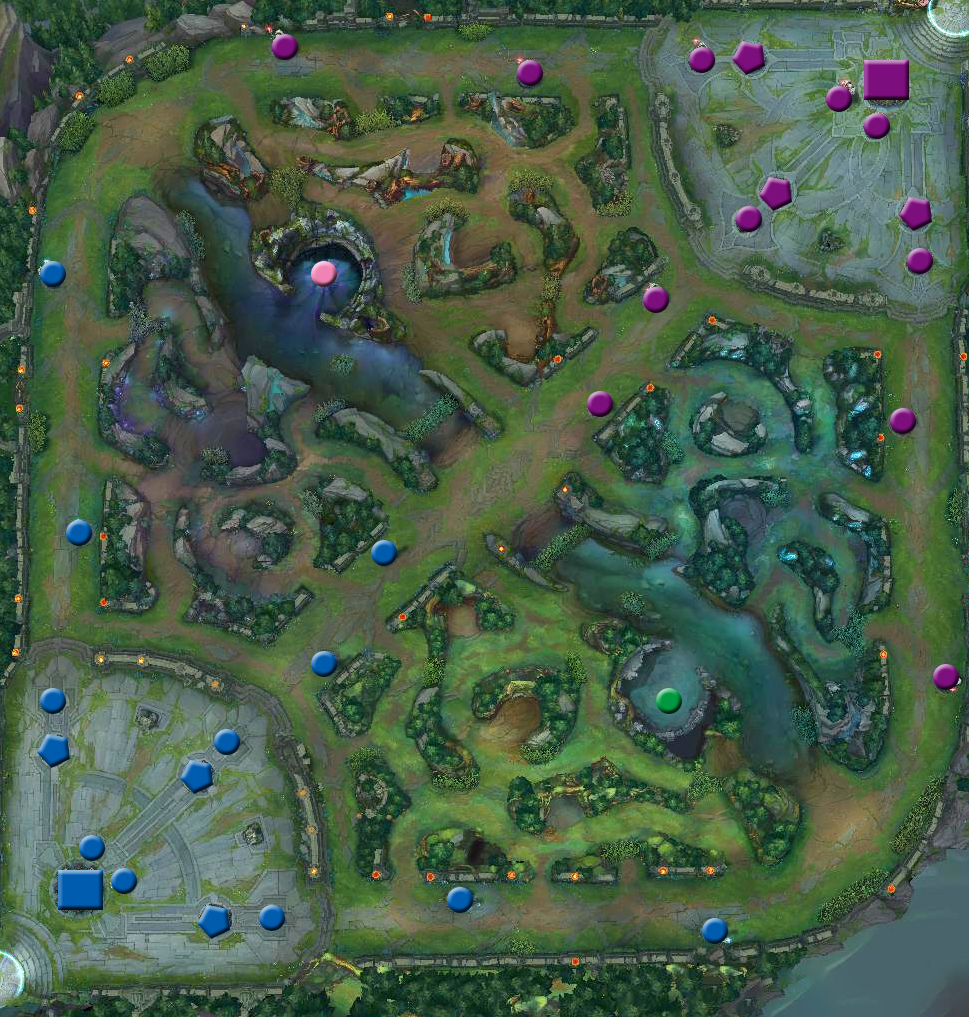
\includegraphics[width=0.6\textwidth]{img/lolmap.jpg}
  \caption{League of Legends map~\cite{lolmap}}\label{fig:lolmap}
\end{figure}

The creeps which are spawned by the nexuses walk toward the opposing teams base, which means they will meet in the middle of the lanes, where the majority of the fighting will take place. Killing the dragon awards the killing team with \emph{dragonslayer}, which makes the champions of the killing team permanently stronger. Killing the baron awards \emph{hand of baron}, makes the killing team significantly stronger for just three minutes.

Experience and gold are the currencies of the game, and they are earned by killing creeps, monsters or opposing champions, both are earned individually by each player. Experience is used to improve the abilities of the champion, while gold is spend purchasing items, that will make the player more powerful. The game is thus an ever-evolving battle of pushing towards the enemies base, winning team fights. Usually one team will accumulate an advantage by being ahead in gold, experience, or both, making their champions stronger and making it easier to win fights. When one team is ahead the other team must play very carefully to have a chance at coming back. 

\begin{figure}[!htb]
  \centering
    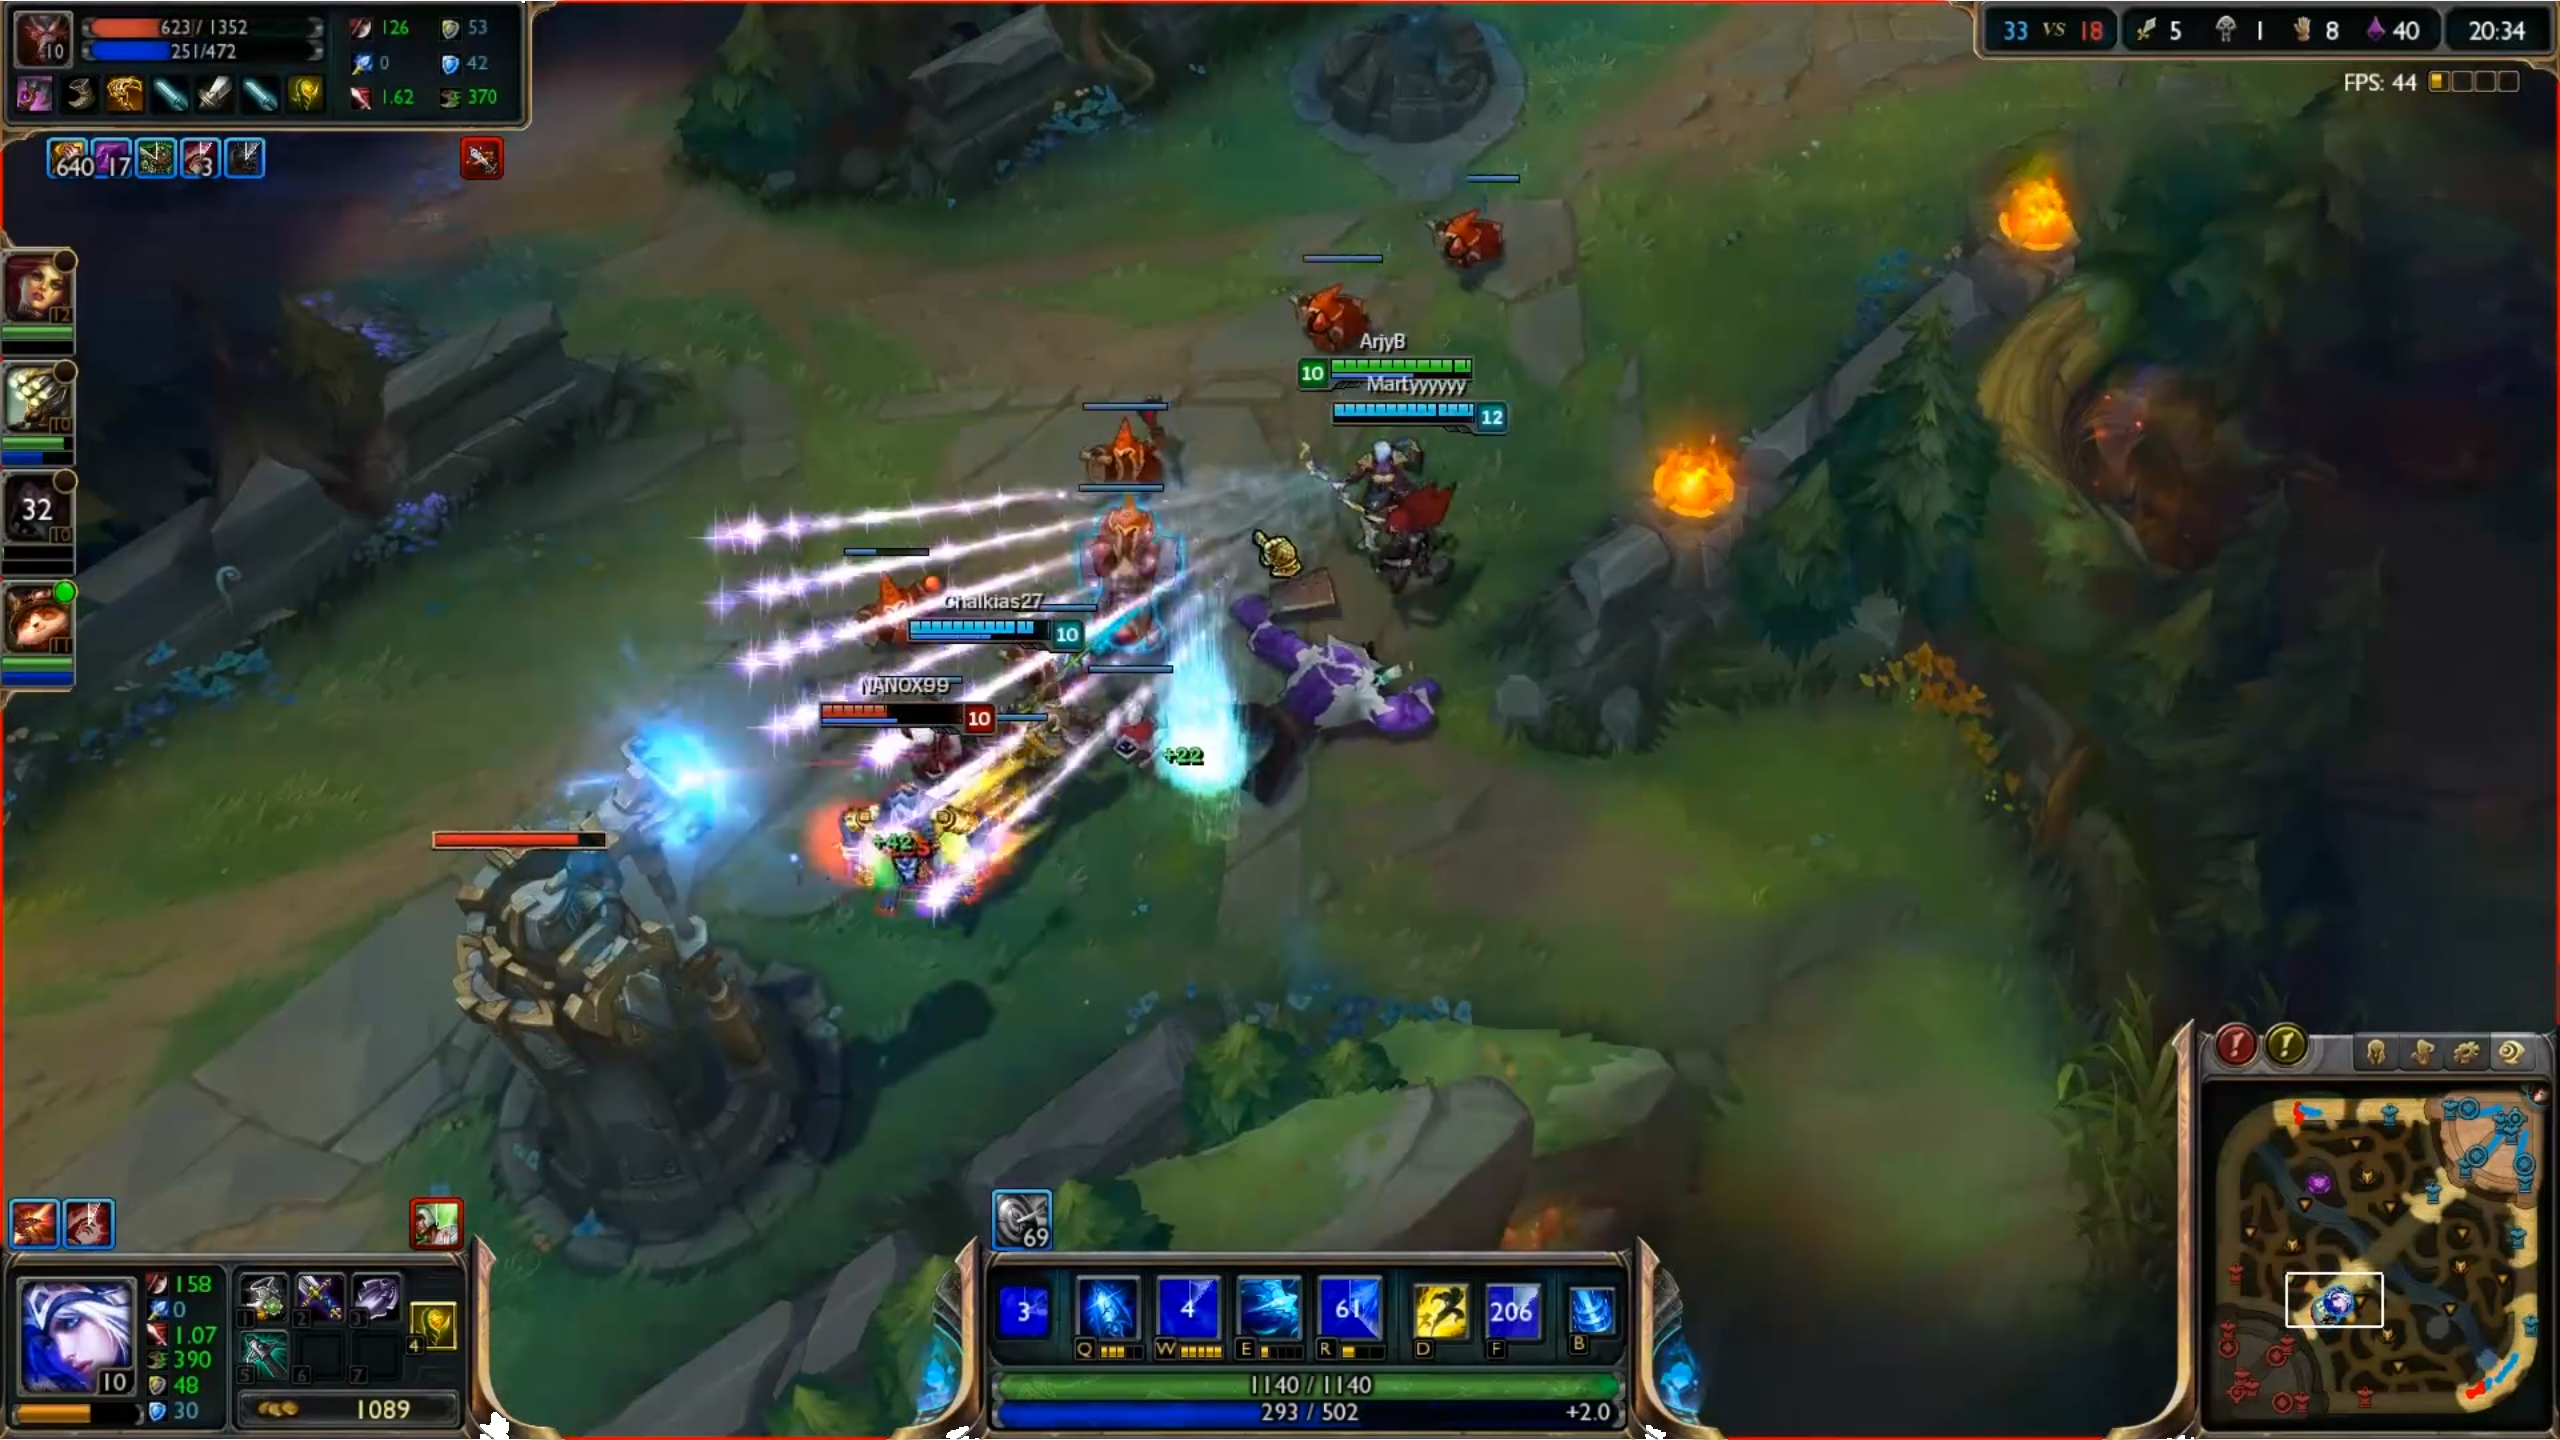
\includegraphics[width=1\textwidth]{img/lolgame.png}
  \caption{Ongoing game: Lower left corner shows Ashes equipment and stats. Upper left corner shows Ashe's team and a summary of the opponents team. Upper right corner shows a score of the game. The lower right corner shows the map including Ashes current position. Lastly in the middle lower screen Ashes abilities and health are shown.}\label{fig:lolgame}
\end{figure}

In \Cref{fig:lolgame}, a screenshot of an ongoing game is presented, here the champion \emph{Ashe} uses \emph{Volley} at an enemy player standing near an enemy turret. The description of a subset of Ashe's skills is shown in \Cref{fig:ashe}, including Volley.

\begin{figure}[!htb]
        \centering
        \begin{subfigure}[b]{0.49\textwidth}
                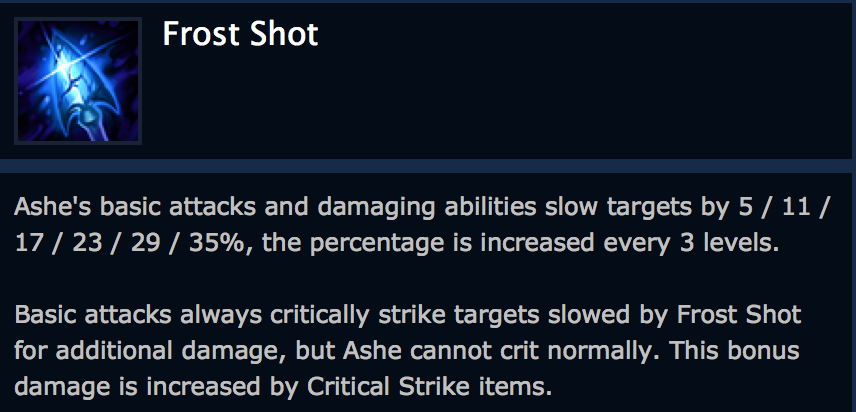
\includegraphics[width=\textwidth]{img/frostshot.png}
                \caption{Example of a passive ability}
                \label{fig:frostshot}
        \end{subfigure}
        %\begin{subfigure}[b]{0.32\textwidth}
        %        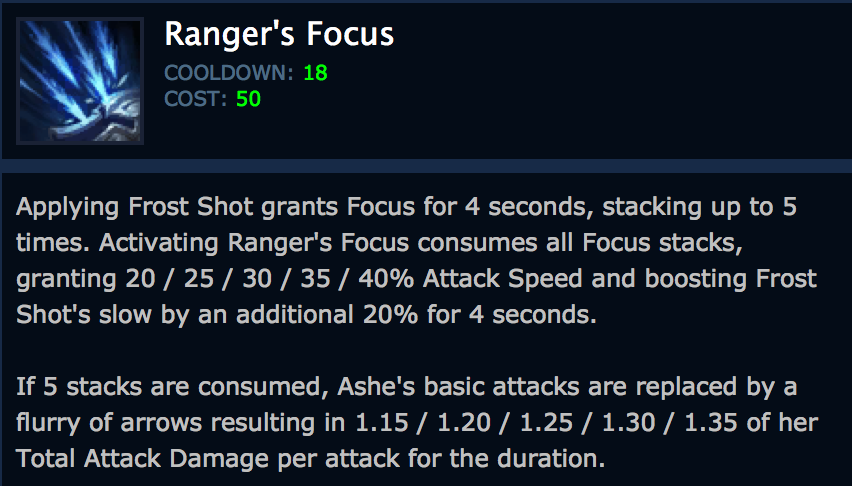
\includegraphics[width=\textwidth]{img/rangersfocus.png}
        %        \caption{}
        %        \label{fig:rangersfocus}
        %\end{subfigure}
        \begin{subfigure}[b]{0.49\textwidth}
                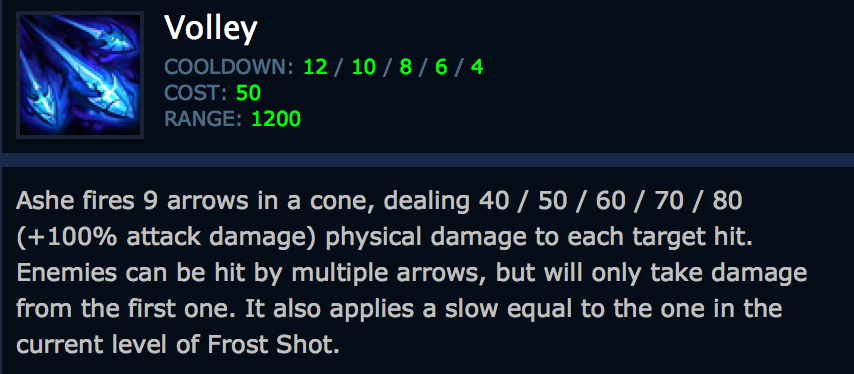
\includegraphics[width=\textwidth]{img/volley.png}
                \caption{Example of an active ability}
                \label{fig:volley}
        \end{subfigure}
        %\begin{subfigure}[b]{0.32\textwidth}
        %        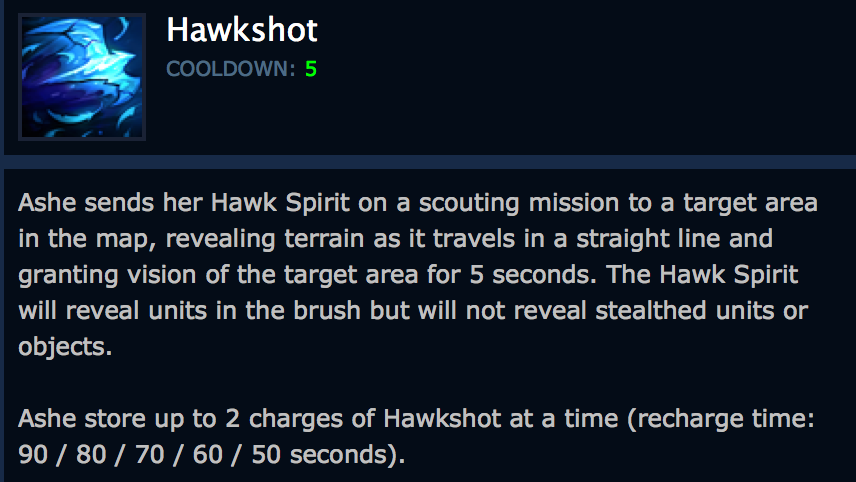
\includegraphics[width=\textwidth]{img/hawkshot.png}
        %        \caption{}
        %        \label{fig:hawkshot}
        %\end{subfigure}
        \begin{subfigure}[b]{0.49\textwidth}
          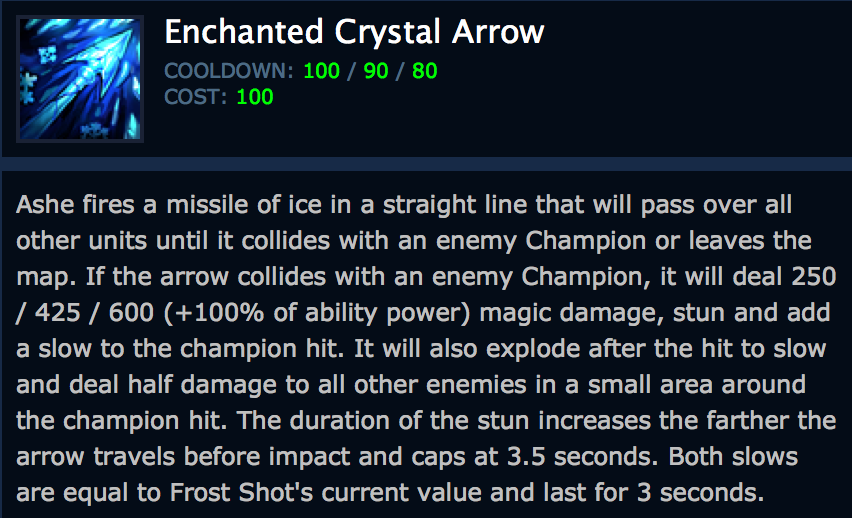
\includegraphics[width=\textwidth]{img/enchanted.png}
          \caption{Example of an ultimate ability}
          \label{fig:enchanted}
        \end{subfigure}
        \caption{Subset of Ashe's skillset~\cite{ashe}}\label{fig:ashe}
\end{figure}

The game combines strategy, individual player skill, communication, and team play. With a prize pool exceeding \$2.000.000 in the 2014 LoL World Championships, the game attracts serious and skilled players~\cite{lolprize}. When playing for such a large sum of money, players want to maximise their ability to win, and we might be able to extract some important knowledge from the game to develop a easy to use method that helps players.

%%% Local Variables:
%%% mode: latex
%%% TeX-master: "../main"
%%% End:
